\section{Security Analysis}\label{sec:security_analysis}
% subsequently shed light on a variety of potential security threats and the possible solutions.

Security is essential for any management systems, and our offloading system is of no exception. 
% The design of our system aims to facilitate the offloading in constrained scenarios, as well as provide a security guarantee. 
In this section, we identify main threats in our proposed architecture. After that, some solutions are proposed to deal with the threats. 

To this end, we use the STRIDE thread model\cite{hernan2006threat} as the security criteria which has six categories: \textbf{S}poofing, \textbf{T}ampering, \textbf{R}epudiation, \textbf{I}nformation disclosure, \textbf{D}enial of service(DoS), and \textbf{E}levation of privilege. Table \ref{tab:threat-property} shows the relations between the threats and the security properties of a system.

\begin{table*}[htbp]
\caption{Threats and Security Properties}
\begin{center}
\begin{tabular}{|p{85pt}||p{65pt}|p{200pt}|}
\hline
Threat & Property & Description \\
\hline
\textbf{S}poofing & Authentication & The identity of users is established.\\
\textbf{T}ampering & Integrity & Data can only be modified by verified person.\\
\textbf{R}epudiation & Non-repudiation & Not denial actions are allowed.\\
\textbf{I}nformation disclosure & Confidentiality & Control the access to the data.\\
\textbf{D}enial of service & Availability  & System is ready for receiving tasks.\\
\textbf{E}levation of privilege & Authorization & Identify the users who can access the data. \\
\hline
\end{tabular}
\label{tab:threat-property}
\end{center}
\end{table*}

Based the model, we list the security threats of our system in Figure \ref{fig:security-analysis} and propose some prevention solutions in the following.
% As shown in Figure \ref{fig:security-analysis}, some components in our system is still susceptible to some security threats.
 \begin{itemize}
\item MEC Server: Overall, the blockchain guarantees the security of MEC servers, specifically, the data integrity and availability.
The authentication process of the blockchain ensures that MEC servers never disclose offloading information. 
In addition, the traceability property of the blockchian prevents the MEC servers from tampering the results of offloading tasks or repudiating their actions.
\item Drone: A malicious drone could spoof (impersonate a normal offloading hub), tamer (change the offloading information during data transmission), repudiate (deny performing an action), DoS (degrade the relay service to IoT devices) or disclose sensitive information of IoT devices.
Signature certification could solve the above potential threats.
Drones could get signed certificates from a MEC server from the blockchain network, and IoT devices could verify the authentication of the offloading hub by those certificates.
\item IoT device: If a trust device is impersonated by a malicious IoT device, it may spread poison content into the offloading system, which consumes the network resources and has a great impact on the performance of task offloading.
The authentication of IoT devices can also avoid the above security threats. 
% Once an IoT device is registered in the system, the drone who manages its offloading request could authenticate its identity.
\end{itemize}


\begin{figure}[t]
\centering
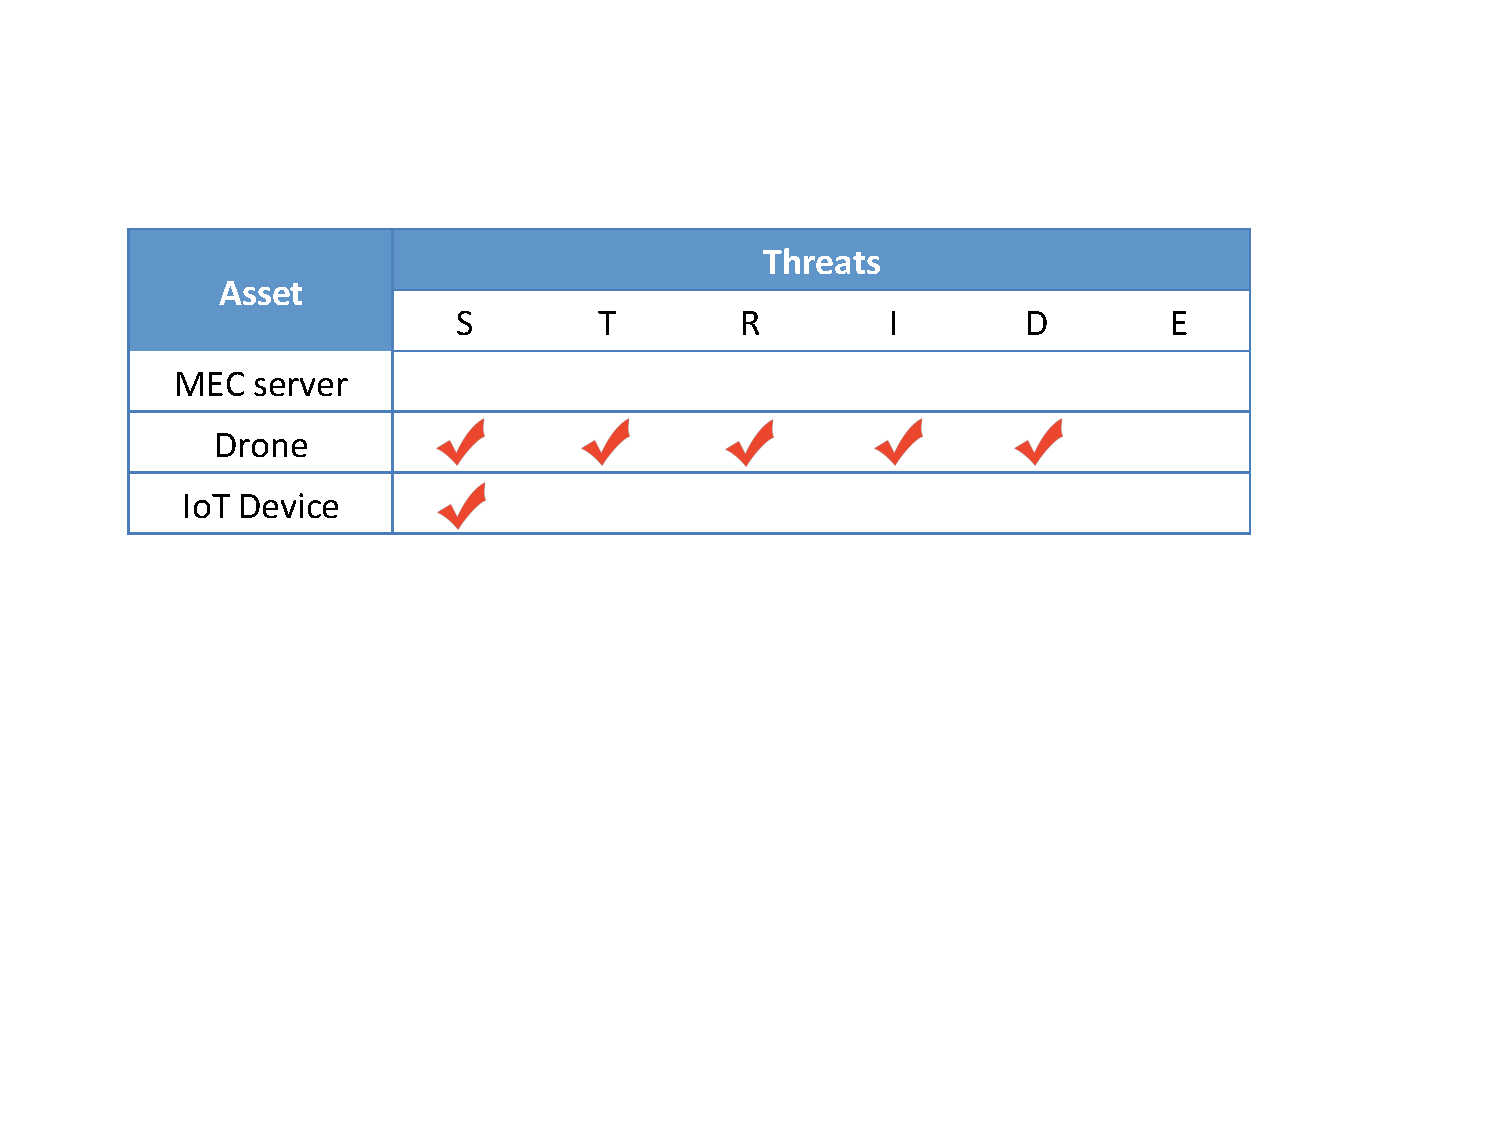
\includegraphics[width=3.3 in]{Fig/SecurityAnalysis.pdf}
\caption{Potential Security Threats}
\label{fig:security-analysis}
\end{figure}

\section{Performance Evaluation}\label{sec:eva}
In this section, we aim to evaluate the feasibility of the proposed architecture which is suitable for any off-loading policy.

\noindent \textbf{Experiment setup.} We implemented the contract in Solidity 0.4.26 \footnote{https://solidity.readthedocs.io/en/v0.4.24/} on the test net of Ethereum network, “Ropsten \footnote{https://ropsten.etherscan.io/}”, which is a popular blockchain test net for evaluation of smart contracts.
Moreover, we emulate a scenario that one drone carries a set of tasks to be offloaded to three MEC servers. 
Four policies discussed in section 3.2 are developed in our smart contract and are used to generate offloading solutions for the submitted tasks.
% For simplicity, we generate four accounts on “Ropsten” to simulate two roles: the drone and MEC servers, where one for the drone and three for MEC servers.

% Since the communication between WSNs and drones is not belonged to the smart contract, we have not implemented that part in our experiment.
% The smart contract focuses on MEC server selection for drones with different offloading policies.
% The smart contract includes four simple offloading policies introduced in section 3.2, the Random policy, the Nearest policy, the MCC policy and the DelayAware policy.
% In our experiment, the account simulated the drone is responsible for the publish of the smart contract, and the other accounts register to the smart contract.
% All registered accounts can communicate with the interfaces to capture or transmit the related information.

In our smart contract, we define an interface $GetTaskInfo()$ to capture the task information, including data amount, computation amount and ID, meanwhile anther interface $GetServerInfo()$ is defined to obtain the MEC server information, such as MEC-Drone distance, computation capacity and address.
% In order to compare the cost of various offloading policies, we define four interfaces to conduct the corresponding policies, i.e., the random policy, the nearest policy, the MCC policy and the DealyAware policy.

\noindent \textbf{Evaluation metrics.}
We measure the performance of the policies via ``Gas'' which is the cost for the miners to execute the transactions. This cost depends on the complexity of each policies, i.e., how much computation and storage resources are consumed for running the smart contract. Each experiment is repeated 20 times, and the average values and their variance are reported.

% The complexity of each interface in the smart contract depends on the its required computation and storage resource.
% Since the interface needs the miner to invoke, more payment to the miner is required with more complex interface to  be executed.
% The payment to the miner is called the transaction fee, measured as “Gas” defined in Ethereum, which is a unit to evaluate the miner‘s work amount when it executes the transaction.
% Hence, we record the gas consumption of each interface with the increase number of offloading tasks. 


Figure \ref{fig:Gas} demonstrates the experimental results, where the DelayAware policy consumes more gas than others with the increasing number of tasks.
For convenience of analysis, the number of offloading tasks is assumed as $n$, while the number of MEC servers is represented as $m$.
The reason is that the time complexity of the DealyAware policy is $O(2n+m)$, relatively simpler than other policies, i.e., the random policy is in $O(n)$ time, the Nearest policy and MCC policy are the same with the time complexity of $O(n+m)$.
In this experiment, $m$ is a constant, equal to 3.
Hence, the gas consumption of all four policies is linearly increasing with the number of offloading tasks.

\begin{figure}[t]
\centering
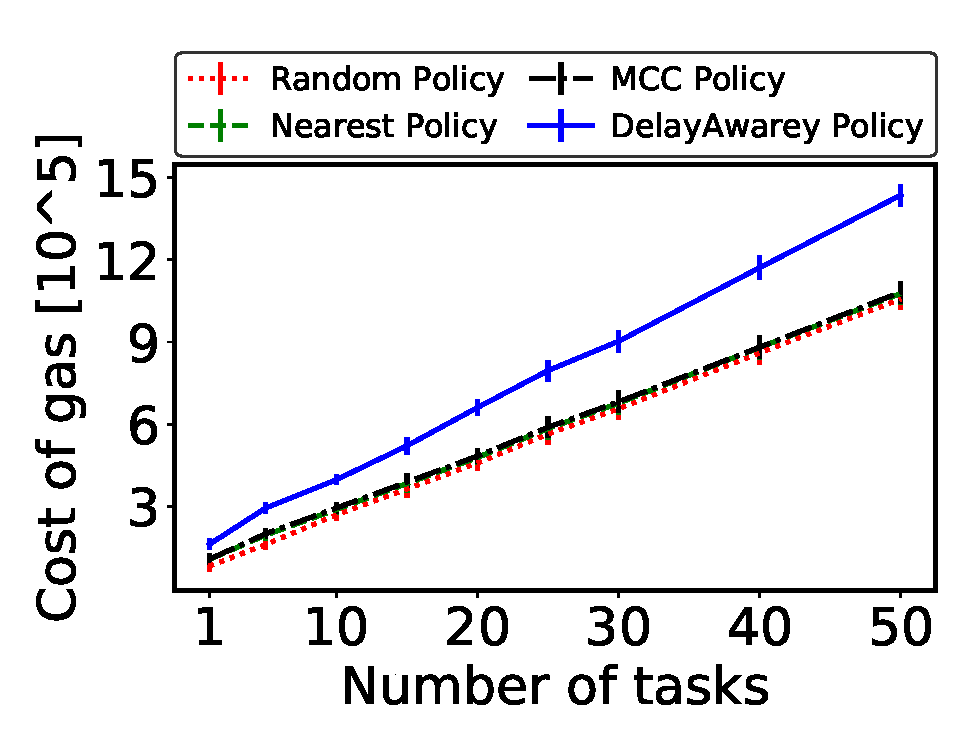
\includegraphics[width=3in]{Fig/PolicyGas.pdf}
\caption{The Gas Consumption under Different Offloading Policies}
\label{fig:Gas}
\end{figure}

